% TEMPLATE for Usenix papers, specifically to meet requirements of
%  USENIX '05
% originally a template for producing IEEE-format articles using LaTeX.
%   written by Matthew Ward, CS Department, Worcester Polytechnic Institute.
% adapted by David Beazley for his excellent SWIG paper in Proceedings,
%   Tcl 96
% turned into a smartass generic template by De Clarke, with thanks to
%   both the above pioneers
% use at your own risk.  Complaints to /dev/null.
% make it two column with no page numbering, default is 10 point

% Munged by Fred Douglis <douglis@research.att.com> 10/97 to separate
% the .sty file from the LaTeX source template, so that people can
% more easily include the .sty file into an existing document.  Also
% changed to more closely follow the style guidelines as represented
% by the Word sample file. 

% Note that since 2010, USENIX does not require endnotes. If you want
% foot of page notes, don't include the endnotes package in the 
% usepackage command, below.

\documentclass[letterpaper,twocolumn,12pt]{article}
\usepackage{usenix,epsfig,endnotes}
\usepackage[]{graphicx}
\usepackage[sort, numbers]{natbib}
\usepackage{hyperref}
\usepackage{adjustbox,lipsum}
\usepackage{subfig}

\title{\Large \bf GeoSched: Minimizing Cost of Cloud Workloads in Geo-Distributed Data Centers} 
\author{
{\rm Anirudh Jayakumar}\\
University of Illinois at Urbana-Champaign
\and
{\rm Harshit Dokania}\\
University of Illinois at Urbana-Champaign
} % end author

\newenvironment{list1}{
  \begin{list}{\ding{113}}{%
      \setlength{\itemsep}{0in}
      \setlength{\parsep}{0in} \setlength{\parskip}{0in}
      \setlength{\topsep}{0in} \setlength{\partopsep}{0in}
      \setlength{\leftmargin}{0.17in}}}{\end{list}}
\newenvironment{list2}{
  \begin{list}{$\bullet$}{%
      \setlength{\itemsep}{0in}
      \setlength{\parsep}{0in} \setlength{\parskip}{0in}
      \setlength{\topsep}{0in} \setlength{\partopsep}{0in}
      \setlength{\leftmargin}{0.2in}}}{\end{list}}

  \begin{document} 
  \maketitle 


\subsection*{ABSTRACT}
Today, many of the leading cloud service providers have geographically distributed data centers to serve millions of users around the world. The need for a geo-distributed data center arises from the need to provide low-latency and  high-availability of the different services. The workloads that run on these data centers are also highly diverse. A typical data centers run jobs of different kinds including business-critical workloads---web servers, mail servers, instant messaging services etc, big-data processing, real-time data analytics and HPC jobs. As cloud services grow to serve more customers, there is an increasing need for a workload provisioning mechanism which can minimize the cost of operation of the data center while minimizing SLA violations and also minimizing the user-perceived latency. 

We present GeoSched, a job provisioning framework that is workload aware, energy-aware and cooling-aware. GeoSched considers the workload type (batch process, real-time processing, web-service), the energy source of the data center (brown and green energy), electricity pricing of the region and cooling techniques used in the data center (air economizer). We GeoSched on industry workload traces and also on synthetic workloads that can mimic the real-world data center workload. 

\section{INTRODUCTION}
\label{sec:intro}

\textbf{Problem Statement:} Minimize the total cost of operations of a geo-distributed data center running cloud workloads by minimizing the energy costs subject to business constraints like the service level agreement(SLA) and other technical constraints like data center capacity limits. The energy costs will depend on the power usage of the IT infrastructure and also the energy required by the cooling infrastructure to maintain the desired temperature inside the data center. Additionally, the solution should also consider the different energy source(green and brown) available at the data center and the different workload types that are typical to a cloud data center.


%%%%%%%%%%%%%%%%%%%%%%%%%%%%%%%%%%%%%%%%%%%%%%%%%%%%%%%%%%%%%
\section{RELATED WORK}
\label{sec:related} 
Cost minimization has been extensively studied both in the context of a single data center and a geo-distributed data center. Most of the work has been targeted towards minimizing the energy consumption of the data center to reduce the operational cost. For example, the work by Gu et al. \cite{gu2014cost} studies the influence of task assignment, data placement  and data movement on the operational expenditure of large-scale geo-distributed data centers for big data applications. The authors jointly optimize  these three factors by proposing a 2-D Markov chain to derive the average task completion time and solve the model as a MILP problem. On similar lines Agarwal et al. \cite{agarwal2010volley} propose an automated data placement mechanism Volley for geo-distributed cloud services with the consideration of WAN bandwidth cost, data center capacity limits, data inter-dependencies, etc. 

Yu et all.\cite{yu2015energy} propose minimizing energy cost for distributed Internet data centers (IDCs) in smart microgrids by considering system dynamics like uncertainties in electricity price, workload, renewable energy generation, and power outage state. They model the problem as a stochastic program and solve it using Lyapunov optimization technique. The work by Ren and He  \cite{ren2013coca} propose an online algorithm, called COCA to minimize data center operational cost while satisfying carbon neutrality. Unlike some of the existing research, COCA enables distributed server-level resource management: each server autonomously adjusts its processing speed and optimally decides the amount of workloads to process. This work is restricted to a single data center with heterogeneous resources. 

Cooling energy is a substantial part of the total energy spent by a data center. According to some reports, this can be as high as 50\% \cite{sullivan2002alternating}, \cite{patel2003smart},\cite{sawyer2004calculating} of the total energy budget. There has been a lot of work both at the application/middleware level \cite{TempLDBSC11}, \cite{leverich2010energy} as well as provisioning techniques  \cite{tang2007thermal}, \cite{chen2010integrated} that try to minimize the cooling energy. Li et all. \cite{li2014coordinating} proposes SmartCool, a power optimization scheme that effectively coordinates different cooling techniques and dynamically manages workload allocation for jointly optimized cooling and server power. Unlike existing work that addresses different cooling techniques in an isolated manner, SmartCool integrates different cooling systems as a constrained optimization problem. Also, since geo-distributed data centers have different ambient temperatures, SmartCool dynamically dispatches the incoming requests among a network of data centers with heterogeneous cooling systems to best leverage the high efficiency of free cooling.  

\iffalse


Other research related to cooling efficiency include the work by Liu et all \cite{liu2012renewable}  that reduces electricity cost and environmental impact using a holistic approach that integrates renewable supply, dynamic pricing, and cooling supply including chiller and outside air cooling, with IT workload planning to improve the overall sustainability of data center operations. The authors first predict renewable energy as well as IT demand. Then they use these predictions to generate an IT workload management plan that schedules IT workload and allocates IT resources within a data center according to time varying power supply and cooling efficiency. Pakbaznia and Pedram \cite{pakbaznia2009minimizing} focuses on minimizing power for both IT equipment and air conditioning power usage. The authors consider both server consolidation and task assignment together and formulate the resulting optimization problem a a ILP problem and present a heuristic algorithm that loves it in polynomial time.

There are also research done to look at the impact of failures in data centers on the operational cost. The work by Cui et al. \cite{cui2014shadows} considers the increase in energy consumption due to failures in large scale clouds. A slower shadow replication of the main process is used to recover from faults thereby saving energy upto 30\%. Guenter et al. \cite{guenter2011managing} also considers different trade-offs between cost, performance and reliability to formulate an optimization problem that minimizes energy costs, reliability costs and unmet demands. VM migration techniques are also used extensively to increase the energy efficiency of cloud data centers. One such approach is proposed by Rodero et al. \cite{rodero2012energy} where the author  propose to use applications€™s profiling (CPU, memory, bandwidth) to  design application-centric energy-aware strategy for VM allocation during VM migration.

Researchers have also studied the efficient use of green energy in data centers. Goiri et al. \cite{goiri2011greenslot} propose a system GreenSlot that maximizes the use of green energy available at data centers while ensuring all job deadlines are met. GreenSlot predicts the solar energy available in data centers in near future and schedules the workload to maximize green energy consumption and meeting jobs€™s deadlines. Green- Slot can increase green energy consumption by up to 117\% and decrease energy cost by up to 39\%, compared to a conventional scheduler. 

\fi

%%%%%%%%%%%%%%%%%%%%%%%%%%%%%%%%%%%%%%%%%%%%%%%%%%%%%%%%%%%%%


%%%%%%%%%%%%%%%%%%%%%%%%%%%%%%%%%%%%%%%%%%%%%%%%%%%%%%%%%%%%%


\section{CLOUD WORKLOADS } 
With the increase in the adoption of cloud computing by businesses around the world, more and more workloads are moving out of traditional data centers into the cloud. A cloud data center typically handles a range of IT workloads. These workloads include service-critical and latency sensitive interactive applications that run 24x7 such as instant messengers, e-mail applications and other internet services, and batch-style applications such as scientific HPC applications, BigData applications like financial analysis and MapReduce applications. A thoughtful management of these workloads are necessary not only to provide customers with low-latency services but also to reduce the energy consumption of the data centers that run these workloads. A good way to study these workloads are by analyzing real-world or synthetic workload traces. We look at cloud workload traces in detail in section \ref{traces} and \ref{googletrace}

\subsection{Workload Traces} \label{traces}
Unfortunately, there is a lack of real-world traces in the cloud computing research community. As a result, there are limited work done to understand the diversity in cloud workloads. The first large-scale workload trace was released by Google in 2011\cite{googletracedata}, featuring traces from over 12,000 servers over a period of 29 days. Various studies have been carried out to understand the characteristic of the Google trace data. Other real-world traces include Wikipedia request trace \cite{urdaneta2009wikipedia} and Hadoop logs from Yahoo! \cite{yahootrace}There have also been attempts to generate synthetic workload traces using known real-world workload characteristics \cite{beitch2010rain} \cite{wang2011towards}. For our experiments we have decided to use the workload trace from Google. 

\subsection{Custom Trace Format}
To have a common trace format to represent different real-world and synthetic workload traces, we have formulated a trace format similar to standard workload format (swf) \cite{chapin1999benchmarks} defined for grid and supercomputing traces. Table \ref{tab:format} provides information about each field int the trace format.
 
\begin {table}[]
\centering
 \scalebox{0.7}{\begin{tabular}{ | p{3cm} |l  |p{6 cm}|  }
    \hline
    \bf{Field Name} & \bf{Type} & \bf{Description}   \\ \hline
     JobID & INT  & Unique job identifier for each job\\ \hline
     Arrival Time & INT & Arrival time in microseconds \\ \hline
     Scheduled Time & INT  & Arrival time in microseconds\\ \hline
     Finish Time & INT  & Arrival time in microseconds\\ \hline
     Schedule class & INT  & Latency class of the job. \\ \hline
     Tasks & INT  & Total number of tasks in the job. \\ \hline
     Total CPU& INT  & Aggregate sum of CPU used by all the tasks in the job\\ \hline
     Total Memory& INT   & Aggregate sum of memory used by all the tasks in the job \\ \hline
     User& INT  & Unique user identifier \\ \hline
     SLA Param1&  FLOAT & SLA parameter placeholder\\ \hline
     SLA Param2&  FLOAT & SLA parameter placeholder\\ \hline
     SLA Param3&  FLOAT & SLA parameter placeholder\\ \hline
    \end{tabular}}
    \caption {Trace format description} \label{tab:format} 
\end{table}

\subsection{Google Workload Trace} \label{googletrace}
Google trace has job and task information in different files. We consolidated all the required information and generated a single work trace file with the format described in the previous section. For our work, we model five different data centers located at different parts of the globe. A detailed explanation about the data center profile are given in section \ref{sec:datacenter}. To simulate workload execution in these five data centers we have extracted five set of traces each worth five days of incoming job requests from the original google trace. This will cover 25 days of traces out of the 29 available days. We label these 5 set of traces from A to E. Additionally, in our experiments we only consider those jobs that end without any failures. Therefore, we clean the original traces by removing all jobs that is either fail or get killed. 

\begin{figure}[] 
\centering
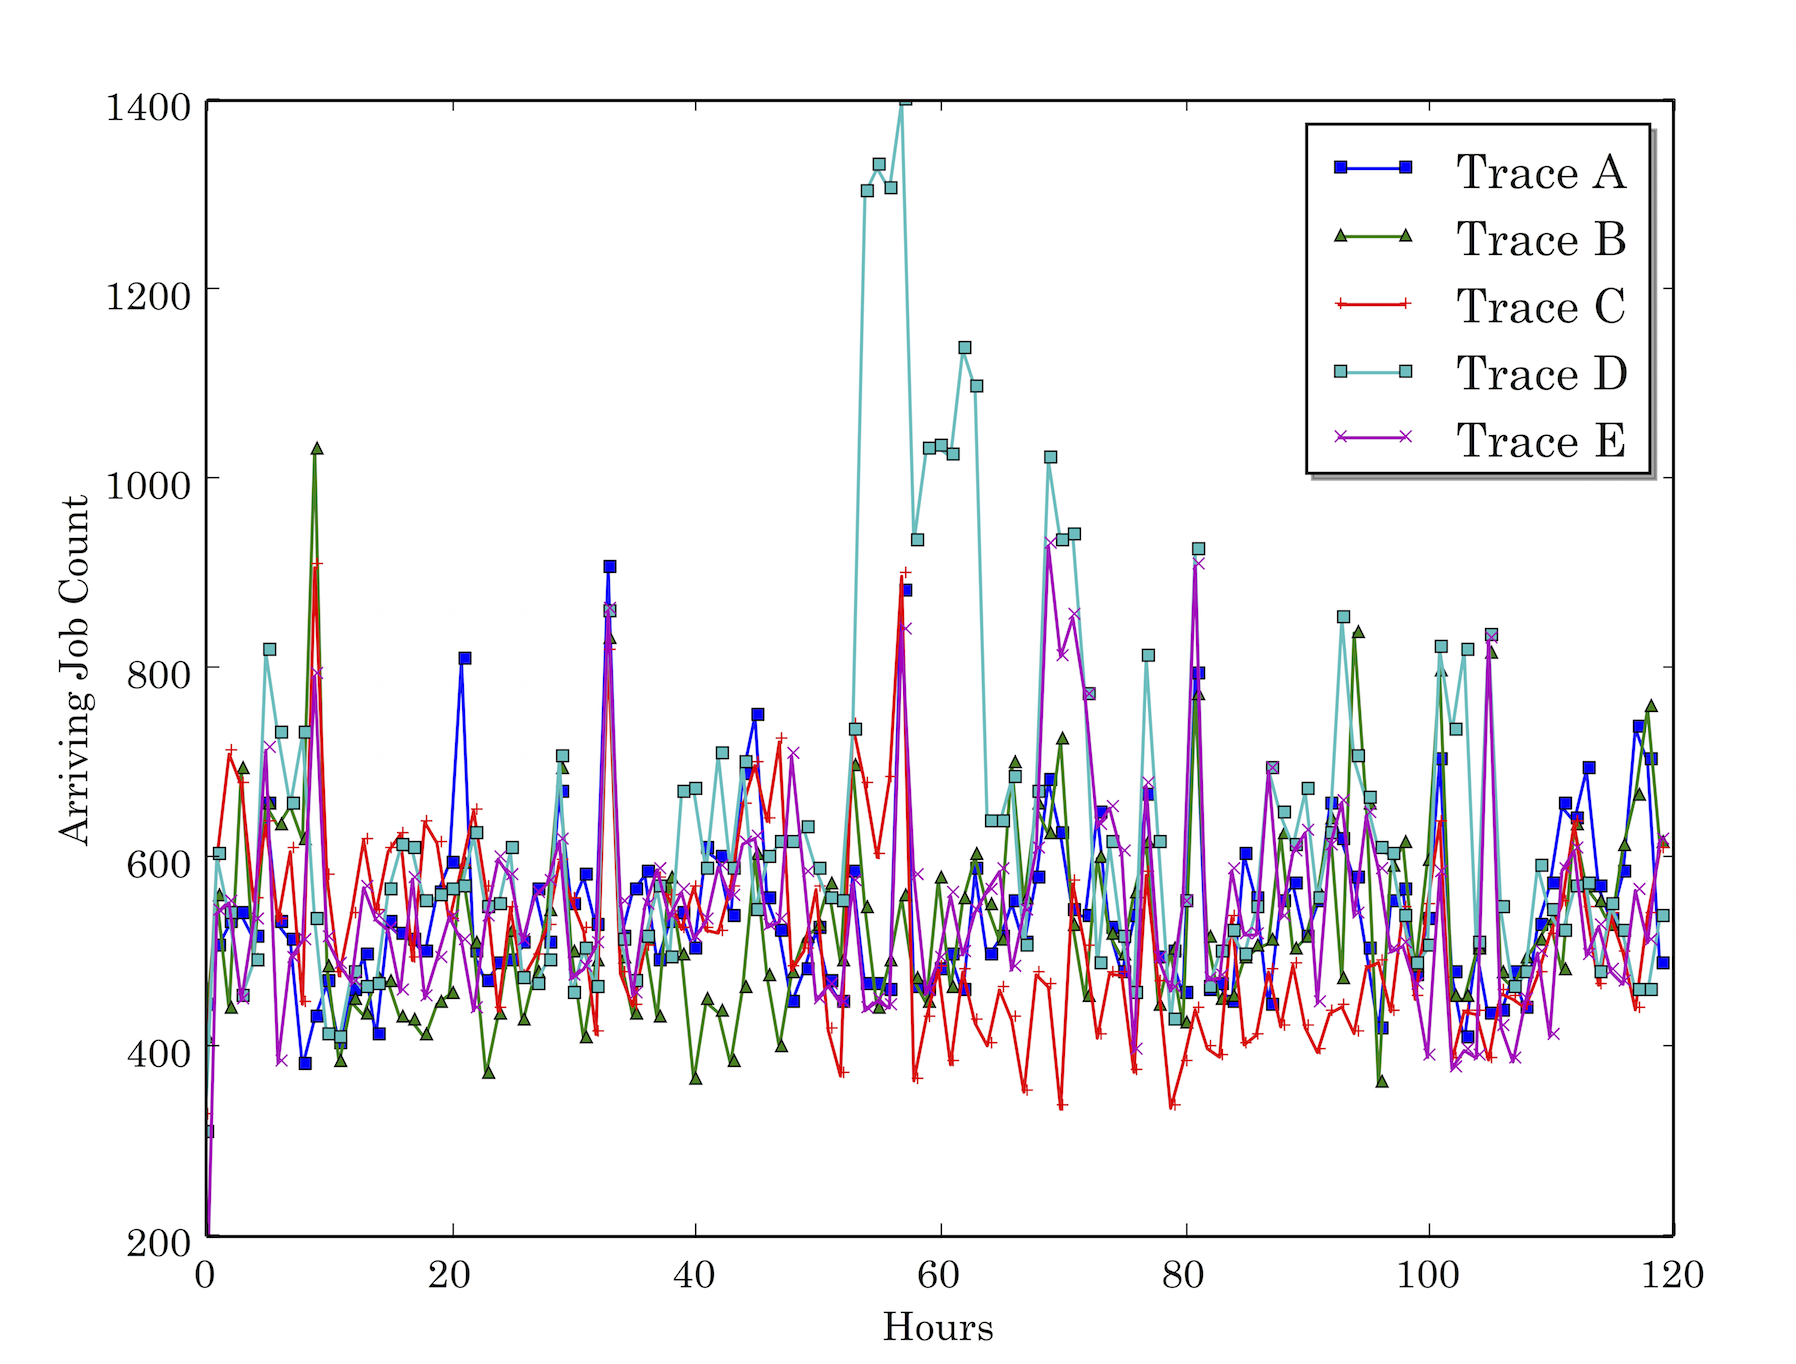
\includegraphics[scale=0.25]{arrivalrate.png}
\caption{Arrival rate of jobs }
\label{fig:arrivalrate}
\end{figure}

Now we will look at some characteristics of the traces. Table \ref{tab:tracestat} describes the statistics for each of the five traces grouped by the scheduling class of the job. In google traces, CPU and memory usage are normalized relative to the largest capacity of the resource on any machine in the trace (which is 1.0). Most of the class 0 and class 2 jobs are batch jobs with less latency requirements. Generally, these are the kind of jobs that can be provisioned on other data centers as their deadlines are not strict.  You will find that as the sensitivity increases the running time of these jobs and the resource usage also increase. High-sensitive jobs are generally service jobs and run of longer periods of time. Figure \ref{fig:pie} shows a pie chart of the job counts in different schedule classes for all the 5 traces. You will notice that the job count for class 3 (high latency-sensitive) jobs are low. This is because these jobs generally run for long period of time, typically months. Since we only consider jobs that start and end within the 29 day range such jobs are missed out in our traces. For our work, we will consider class-0 and class-1 jobs as candidates for optimizing the provisioning. We leave, class-2 and class-3 jobs to run on the data center where the job arrived since these are high-sensitive and their SLA demands will be strict.


\begin{figure*}[]
\centering
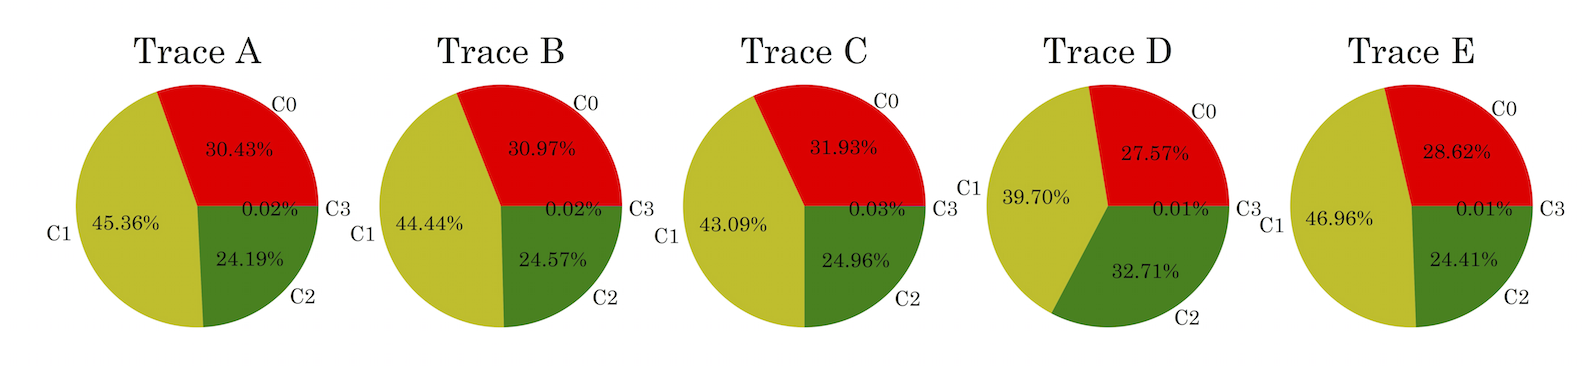
\includegraphics[scale=0.65]{pie}
\caption{ Distribution of job count in various schedule classes}
 \label{fig:pie}
\end{figure*}

\begin{table*}
\adjustbox{max width=1\textwidth}{

\begin{tabular}{|l|l|l|l|l|l|l|l|l|l|l|l|l|l|l|l|}
\hline
 & \multicolumn{3}{l|}{\bf{Trace A}} & \multicolumn{3}{l|}{\bf{Trace B}} & \multicolumn{3}{l|}{\bf{Trace C}} & \multicolumn{3}{l|}{\bf{Trace D}} & \multicolumn{3}{l|}{\bf{Trace E}} \\ \hline
\textbf{\begin{tabular}[c]{@{}l@{}}Sched\\ Class\end{tabular}} & \textbf{\begin{tabular}[c]{@{}l@{}}Avg \\ CPU\end{tabular}} & \textbf{\begin{tabular}[c]{@{}l@{}}Avg\\ Mem\end{tabular}} & \textbf{\begin{tabular}[c]{@{}l@{}}RT\\  (secs)\end{tabular}} & \textbf{\begin{tabular}[c]{@{}l@{}}Avg\\ CPU\end{tabular}} & \textbf{\begin{tabular}[c]{@{}l@{}}Avg\\ Mem\end{tabular}} & \textbf{\begin{tabular}[c]{@{}l@{}}RT\\  (secs)\end{tabular}} & \textbf{\begin{tabular}[c]{@{}l@{}}Avg\\ CPU\end{tabular}} & \textbf{\begin{tabular}[c]{@{}l@{}}Avg\\ Mem\end{tabular}} & \textbf{\begin{tabular}[c]{@{}l@{}}RT\\  (secs)\end{tabular}} & \textbf{\begin{tabular}[c]{@{}l@{}}Avg\\ CPU\end{tabular}} & \textbf{\begin{tabular}[c]{@{}l@{}}Avg\\ Mem\end{tabular}} & \textbf{\begin{tabular}[c]{@{}l@{}}RT\\  (secs)\end{tabular}} & \textbf{\begin{tabular}[c]{@{}l@{}}Avg\\ CPU\end{tabular}} & \textbf{\begin{tabular}[c]{@{}l@{}}Avg\\ Mem\end{tabular}} & \textbf{\begin{tabular}[c]{@{}l@{}}RT\\  (secs)\end{tabular}} \\ \hline
0 & 0.075 & 0.051 & 415 & 0.123 & 0.096 & 345 & 0.083 & 0.065 & 385 & 0.093 & 0.092 & 373 & 0.093 & 0.074 & 333 \\ \hline
1 & 0.087 & 0.029 & 729 & 0.086 & 0.032 & 760 & 0.082 & 0.028 & 711 & 0.073 & 0.030 & 743 & 0.093 & 0.043 & 693 \\ \hline
2 & 0.067 & 0.043 & 1028 & 0.096 & 0.058 & 872 & 0.088 & 0.057 & 918 & 0.073 & 0.045 & 707 & 0.084 & 0.049 & 832 \\ \hline
3 & 0.088 & 0.12 & 1105 & 0.099 & 0.12 & 82 & 0.101 & 0.012 & 7961 & 0.081 & 0.051 & 17135 & 0.089 & 0.061 & 9021 \\ \hline
\end{tabular}
}
\caption {Trace set statistics} \label{tab:tracestat} 
\end{table*}

Figure \ref{fig:arrivalrate} shows the variation in job arrival rates for the traces. As you can see there is both intra-trace variation as well as inter-trace variation. This is representative of the real-world cloud workload pattern where bursty arrivals are common. There are opportunities to provision jobs to other data centers if the traffic at a particular data center is high. What is also important to notice is that the scheduling decision should be made quickly when the arrival rates of jobs are high, else there are chances for that these jobs miss the SLAs. Hence, even the scheduler should be scalable during high volume traffic. 

Figure \ref{fig:runtime} shows the CDF of the job runtime. As you can see most of the jobs have runtime less than 1024 seconds. This pattern is consistent for all the trace sets. There are a few jobs that have higher run-times. As explained earlier, these jobs are primarily internet-service jobs that are expected to run for longer duration. 


\begin{figure}[] 
\centering
\includegraphics[scale=0.25]{runtime}
\caption{CDF of the job duration}
\label{fig:runtime}
\end{figure}

In google workload trace, it is tough to study the resource usage since these value are scaled down and therefore and accurate picture of the resource utilization is tough to generate. In figure \ref{fig:resource} we can see that most jobs request a small portion of the cluster resources. Most of the resources in the google cluster are used by the few service jobs that are present. The large number of batch jobs only use a small percentage of the resources \cite{mishra2010towards} \cite{reiss2012heterogeneity}. From the above statistics, we believe that google workload trace provides an accurate representation of the real-world cloud datacenter workload.

\begin{figure} %
    \centering
    \subfloat[CPU resource ]{{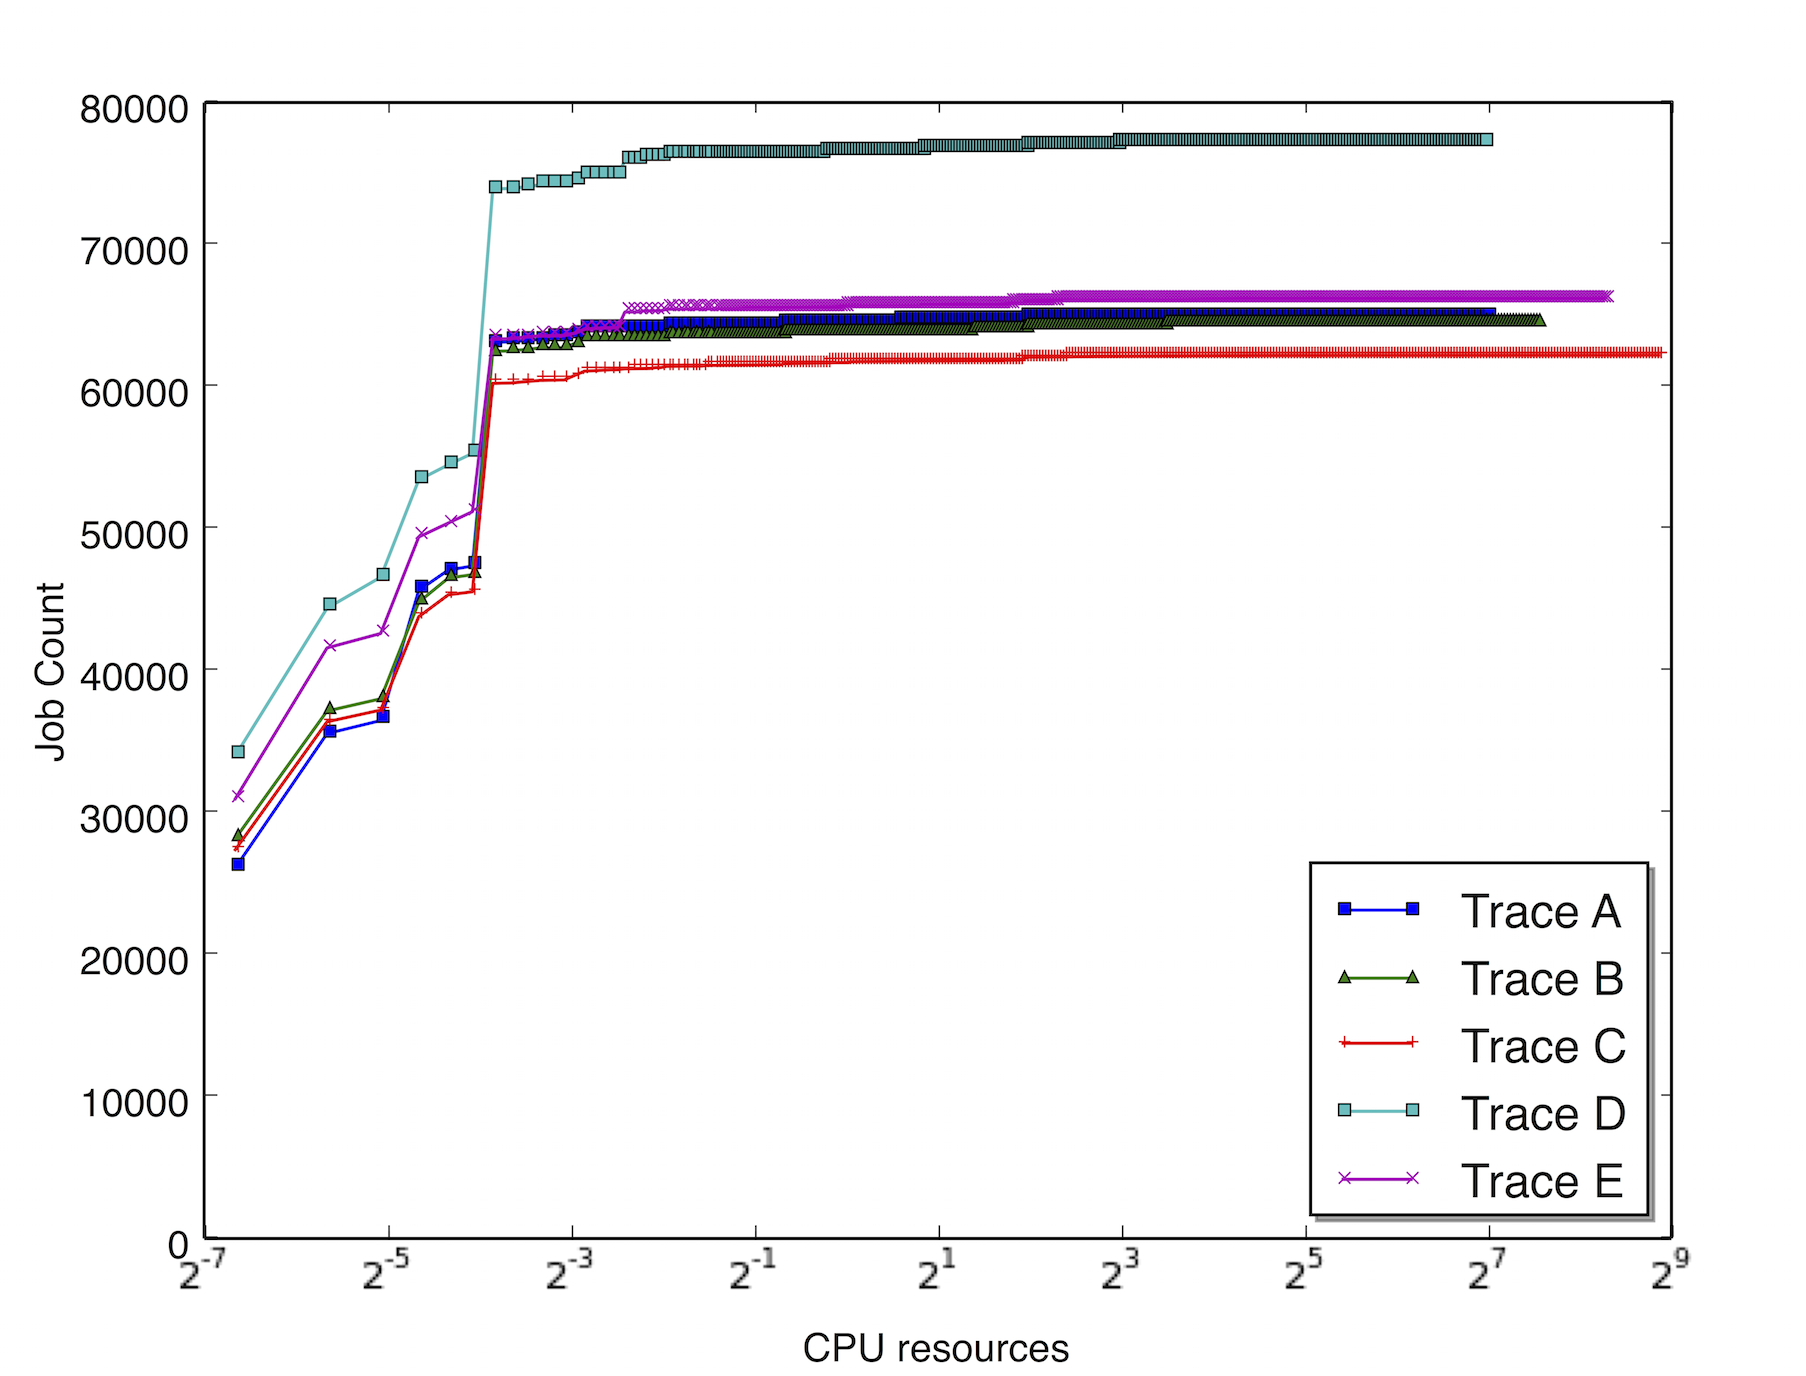
\includegraphics[width=8cm]{cpu} }}%
    \newline
    
    \subfloat[RAM resource]{{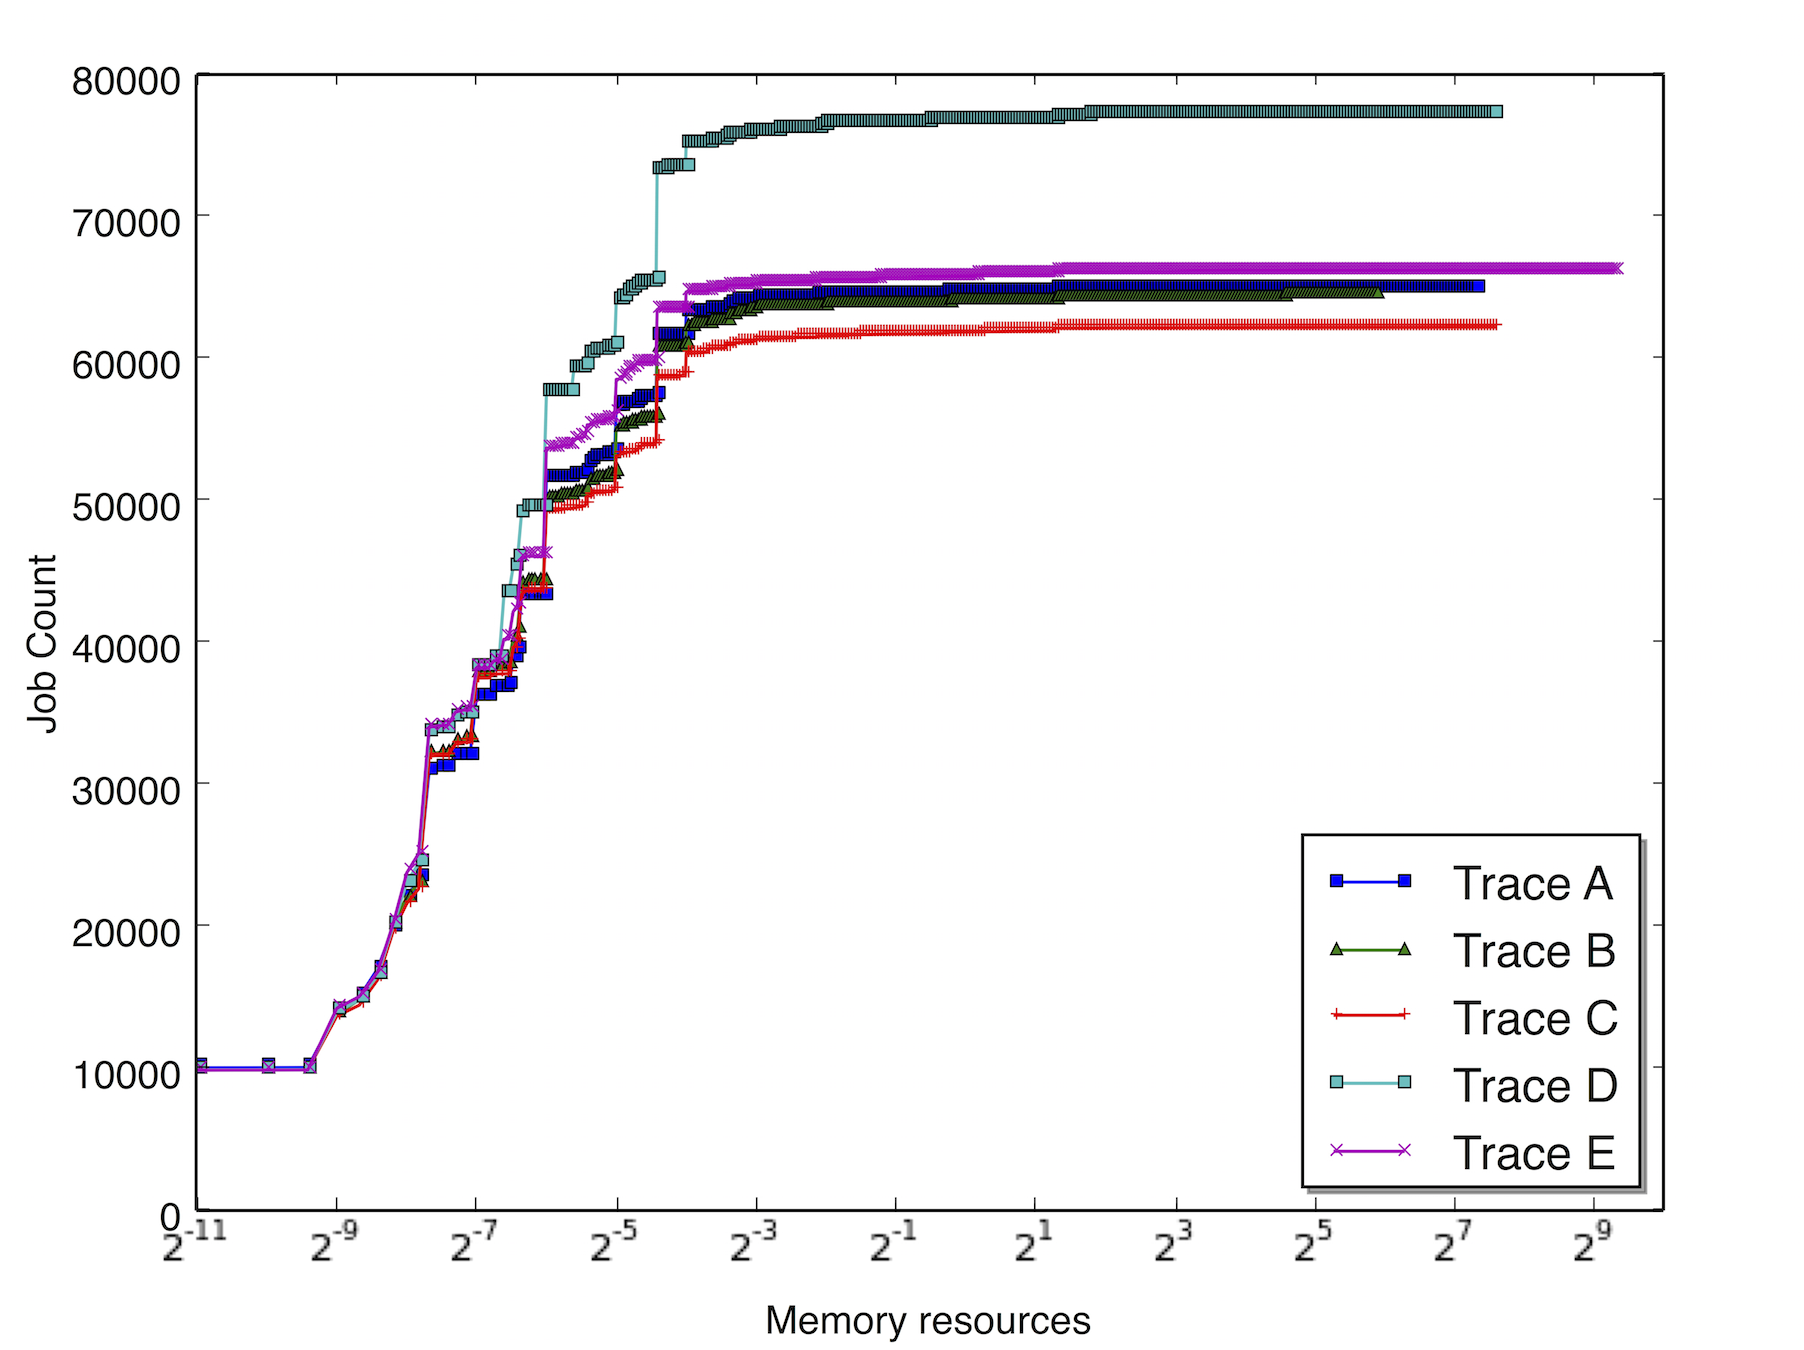
\includegraphics[width=8cm]{mem} }}%
    \caption{CDF of resource requested by jobs}%
    \label{fig:resource}%
\end{figure}

%%%%%%%%%%%%%%%%%%%%%%%%%%%%%%%%%%%%%%%%%%%%%%%%%%%%%%%%%%%%%
\section{DATA CENTER PROFILING } \label{sec:datacenter}
In order to run our experiments, we need to collect information about data centers that will help us make better scheduling decisions. We call this process data center profiling. The major energy costs in data center are from running the IT resources and from cooling the data centers. We create a profile for each of the data center with the information that effects the energy costs.

\begin{table}[] 
 \centering
\begin{tabular}{|p{3cm}|l|p{2.5cm}|}
\hline
\bf{Location}                        & \bf{Label} & \bf{Associated Trace} \\ \hline
Berkeley County, South Carolina & DC1   & A                \\ \hline
Lenoir, North Carolina          & DC2   & B                \\ \hline
Singapore                       & DC3   & C                \\ \hline
Quilicura, Chile                & DC4   & D                \\ \hline
Dublin, Ireland                 & DC5   &   E               \\ \hline
\end{tabular}
\caption {Data center location information} \label{tab:dc}
\end{table}

\subsection{Geo-Distributed Data Center}
Most cloud service providers including Google, Amazon, Facebook and Apple have data centers distributed across the globe. For our experiments, we consider five locations where Google has its data centers\cite{googletracedata}. Table \ref{tab:dc} provides the location and labels for each of the data center. We also replicate the computing resource used in the original google trace across all the data centers. The configuration of the resources along with the normalzed CPU and memory are given in table \ref{tab:dcres}

\begin{table}[] 
 \centering
\scalebox{0.8}{\begin{tabular}{|l|l|l|l|}
\hline
\bf{Node count}      &       \bf{Architecture}          & \bf{CPU} & \bf{Memory} \\ \hline
6732 & B & 0.5 & 0.50   \\ \hline
3863 & B & 0.5 & 0.25   \\ \hline
1001 & B & 0.5 & 0.75   \\ \hline
795 & C & 1 & 1   \\ \hline
126 & A & 0.25 & 0.25   \\ \hline
52 & B & 0.5 & 0.12  \\ \hline
5 & B & 0.5 & 0.3  \\ \hline
5 & B & 0.5 & 0.97  \\ \hline
3 & C & 1 & 0.50  \\ \hline
1 & B & 0.5 & 0.06  \\ \hline
\end{tabular}}
\caption {Data center IT resource configuration} \label{tab:dcres}
\end{table}



\subsection{Profile Parameters}
We consider two major parameters that has the most effect on the energy cost. They are a) Temperature b) Electricity. We collect temperature and electricity prices for these locations from historical archives. If time permits, we wish to also consider green energy available at the data center locations. We look at each of these parameters and how they effect energy costs in sections \ref{sec:temp}, \ref{sec:elec} and \ref{sec:green}.


\begin{figure*} %
    \centering
    \subfloat[Daily Average Temperature ]{{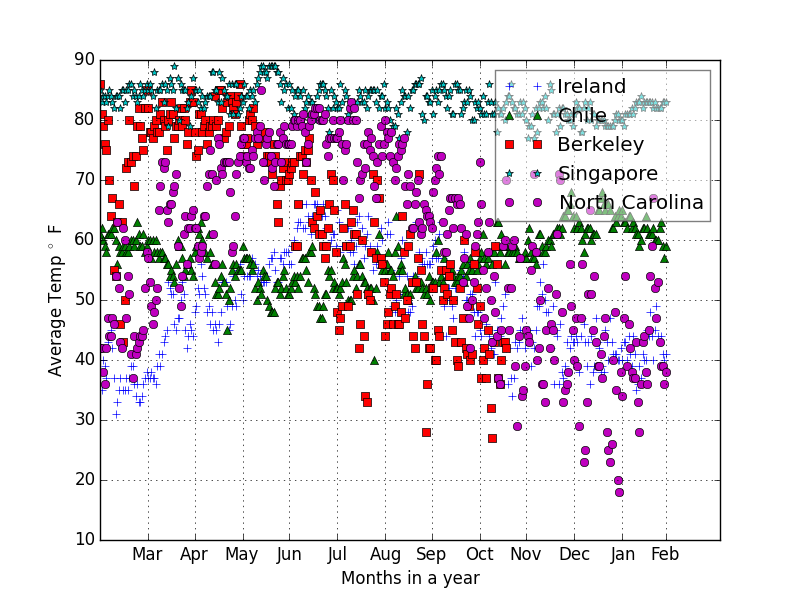
\includegraphics[width=8cm]{AverageTemp} }}%
    \subfloat[Daily Maximum Variation]{{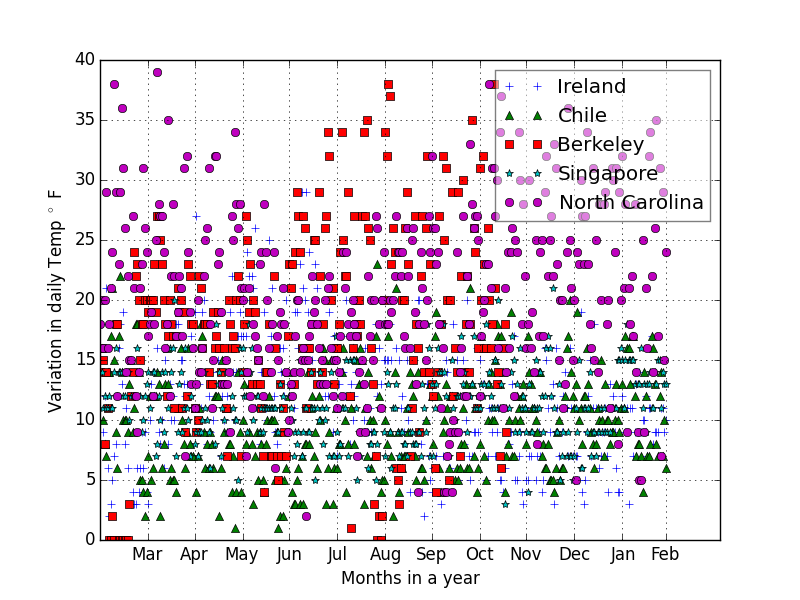
\includegraphics[width=8cm]{Variation} }}%
    \caption{Temperature variation for the year 2013}%
    \label{fig:temp}%
\end{figure*}

\subsubsection{Temperature} \label{sec:temp}
Data centers located in cold regions have the advantage of using outside air to cool the data center. An air-side economizer brings outside air into a building and distributes it to the servers. Instead of being re-circulated and cooled, the exhaust air from the servers is simply directed outside. This can result in million dollars of saving annually. A difference in temperature across data centers mean different cooling costs at these data centers. We wish to utilize this difference by scheduling jobs in low temperature data centers. In this case we make our assumption concrete by doing an empirical analysis of historical climate data. We extracted these historical climate data from various data repositories of the National Climate Data Center \cite{climatedata} for all five locations covering the entire one-year period of 2013.

Figure \ref{fig:temp} a plots the daily average temperature for five different locations in United States, Europe, South-America, and Asia. As expected we see high diversity in temperature at different locations. For example, North Carolina, Ireland seems to be equally favorable for cooling during the month of November {-} March. Chile and Singapore show almost no variation in temperature across the year. However, Chile is favorable for cooling conditions compared to other data centers in the month of May {-} July. 

Figure \ref{fig:temp} b plots the daily maximum variation in temperature across the day i.e. difference of maximum temperature and minimum temperature in a day.  It is worth noting that almost every location faces a variation of up to 40$^{\circ}$F during different periods. These highs and lows do not occur at the same time across different regions due to time differences. It is evident from the results that there is no single location that is always cooling efficient. So we conclude that we need a dynamic scheduler, which caters to the locations that have lower temperature and henceforth save overall energy costs.

\subsubsection{Electricity Pricing} \label{sec:elec}
Creation of power trading zones have resulted in wholesale power purchase under dynamic pricing schemes. Such markets are popular in USA \cite{elecusa}, Germany \cite{elecgermany} and other countries. Based on supply and demand bids there can be high fluctuations in prices \cite{benini2002day}. There are many ways to predict these prices \cite{contreras2003arima} \cite{garcia2005garch}. If we can predict the electricity prices for the job duration, then we will be able to schedule the job such that the running costs go down.

\subsubsection{Energy Source} \label{sec:green}
Solar and wind energy are available in most of the modern data centers. Similar to electricity price predictions green energy prediction can also be done \cite{goiri2012greenhadoop} \cite{aksanli2012utilizing}. Since, this part is in exploratory stage, we will provide more information during the final report.

\subsubsection{Case Study: Google Data Centers} \label{sec:CSgoogle}
Google data-centers show 50\% less energy consumption than a typical data center. Google is able to achieve a trailing twelve-month (TTM) PUE of 1.12 across all data centers, in all seasons, including all sources of overhead.
There are five techniques that Google typically uses to minimize its energy consumption and electricity costs. Frequent measuring of Power Usage Effectiveness is the key for determining the power usage for non-computing functions like cooling and power distribution. Secondly they manage airflow at data-centers, which allows cooling the hot spots available in data-centers. Moreover by setting thermostat to 80$^{\circ}$F it saves significant amount of electricity consumption and costs.


%%%%%%%%%%%%%%%%%%%%%%%%%%%%%%%%%%%%%%%%%%%%%%%%%%%%%%%%%%%%%

\section{SCHEDULER SIMULATOR} 
We plan to implement our simulator using CloudSim \cite{calheiros2011cloudsim}. CloudSim is an extensible simulation toolkit that enables modeling and simulation of Cloud computing systems and application provisioning environments. The CloudSim toolkit supports both system and behavior modeling of Cloud system components such as data centers, virtual machines (VMs) and resource provisioning policies.
\subsection{Components}
\begin{list2} %Job Description%
\item \textbf{Datacenter:} This component will simulate a data center. This composed of 1) scheduler that implements a specific provisioning algorithm, 2) data center profile database, 3) a work trace reader and 4)proxy elements of other data center for inter-data center communication\
\item \textbf{DataCenter Proxy}: All interactions with the data center will be through a proxy. Each datacenter will hold the proxies to other data centers.\
\item \textbf{Scheduler:} This component will implement the optimization technique and schedule jobs onto data centers.\
\item \textbf{Datacenter Profile DB}: This components contains the temperature and electricity data. Scheduler will access this to make provisioning decisions.\
\end{list2}

\begin{figure}[] 
\centering
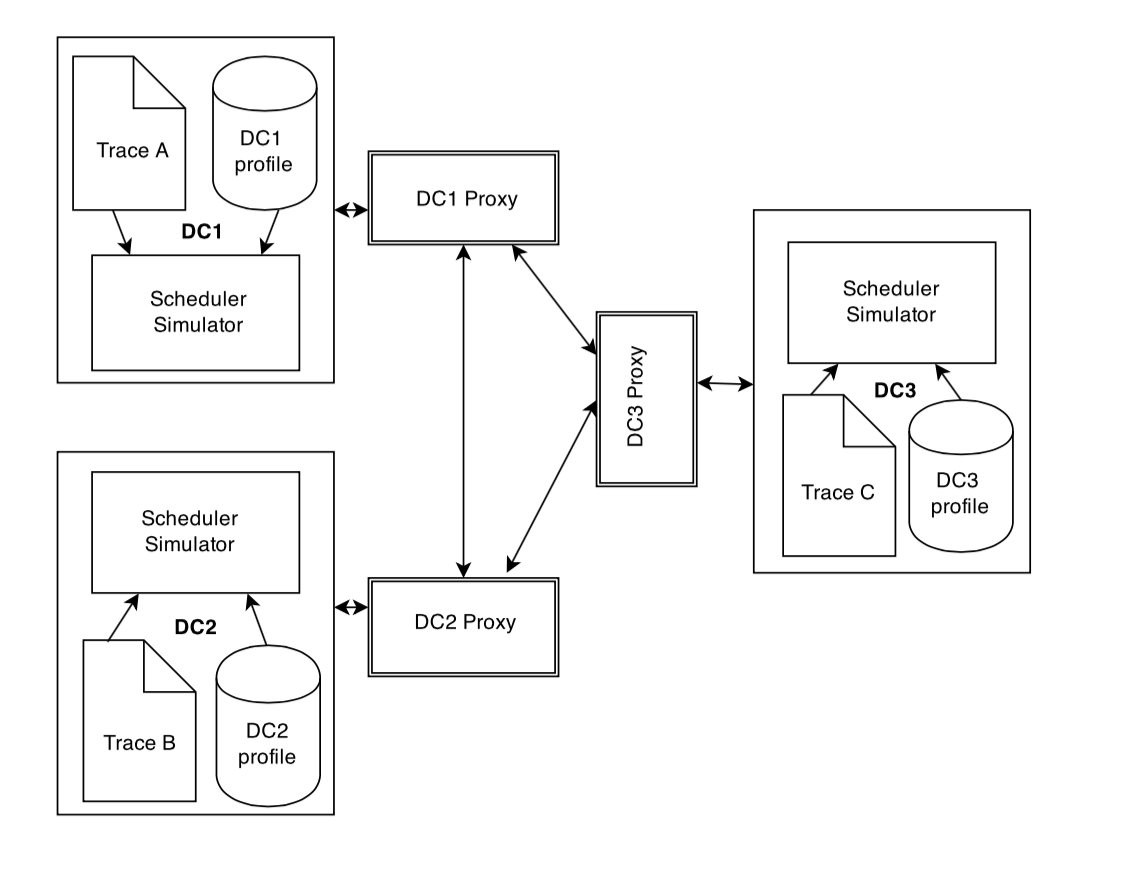
\includegraphics[scale=0.40]{component}
\caption{Simulation components and their interaction}
\label{fig:component}
\end{figure}

\subsubsection{Component Interaction}
Figure \ref{fig:component} gives the interaction model between the components. The datacenter object will start a thread which will run the scheduling algorithm, scheduling jobs from the trace file. Each data center had proxies to other data centers if it needs to communicate resource availability or job provisioning to other data centers.

\section{CONCLUSION}
We have completed the work trace analysis and data center profiling parts of the project. Currently the simulator is being implemented, following which we will work on the energy minimization techniques and the final evaluation of these techniques. If time permits, we would also like to consider green energy in our provisioning mechanism. 
%%%%%%%%%%%%%%%%%%%%%%%%%%%%%%%%%%%%%%%%%%%%%%%%%%%%%%%%%%%%%
\iffalse
\section{SCHEDULING ALGORITHM} 

Provide basic idea about our strategy

\subsection{Features considered}
\subsubsection{Energy Cost Model}
%\subsubsection{Optimization Techiques}
%\subsubsection{Design}
\fi



{\footnotesize \bibliographystyle{acm}
\bibliography{sample}}


\end{document}







